\chapter{User Testing of Prototype}

This chapter describes the methodology and results of user testing conducted on the previously proposed and designed gamification features for English Mind. The testing focused on evaluating the clarity, intuitiveness, and potential engagement effectiveness of the new gamification elements.

Two distinct user groups were selected for testing to provide diverse perspectives. Group A consisted of participants with prior experience using language learning applications, while Group B included participants without significant experience in this area.
\begin{itemize}
    \item \textbf{Group A – Experienced Users}
    \begin{itemize}
        \item 3 participants aged 18-45
        \item Regular users of apps like Duolingo, WordUp, or Duocards
        \item Familiar with gamification concepts through regular usage of language learning applications (even without knowing the formal terminology)
    \end{itemize}

    \item \textbf{Group B – Novice Users}
    \begin{itemize}
        \item 3 participants aged 18-45
        \item Interest in learning English vocabulary
        \item Limited exposure to language learning applications
    \end{itemize}
\end{itemize}

The testing was conducted in a controlled environment where participants interacted with high-fidelity interactive prototypes on mobile devices according to the test scenario (see Section \ref{sec:test-scenario}). During the prototype interaction, participants were encouraged to think aloud, providing real-time feedback on their experience, while observers documented behavioral observations and points of confusion. Afterwards, participants completed a structured questionnaire using a 5-point Likert scale (see Table \ref{tab:questionnaire}) to evaluate feature clarity, perceived usefulness, and engagement potential.

\section{Test Scenario}
\label{sec:test-scenario}
The test scenario was structured as a series of specific tasks that participants were asked to perform, allowing for systematic evaluation of both gamification mechanics and their integration into the learning experience.

The first part of test scenario focused on the streak system understanding:

\begin{enumerate}
    \item Participants were shown the streak status badge and asked to:
    \begin{itemize}
        \item Interpret what the streak status badge represents
        \item Explain how to activate a streak
        \item Describe the requirements for maintaining a streak
        \item Explain what actions would break their streak
        \item Share their thoughts on how the streak system might motivate them
    \end{itemize}
\end{enumerate}
    

In the second part of test scenario participants were asked to complete a practice session with various flashcard types:
\begin{enumerate}
    \item For each flashcard type, they were instructed to:
    \begin{itemize}
        \item Read the instructions aloud
        \item Explain how they would interact with the card
        \item Complete the task while verbalizing their thought process
    \end{itemize}

    \item After completing several flashcards, participants were asked to:
    \begin{itemize}
        \item Identify and explain the purpose of the element located in the top-right corner of the screen (without being told it was a progress tracker)
        \item Describe stage system of the vocabulary progress tracker
        \item Share how seeing their it affects their motivation
    \end{itemize}

    \item At the end of the practice session, participants were asked to:
    \begin{itemize}
        \item Interpret their practice statistics
        \item Explain how the session completion affects their streak
        \item Share their reaction to the celebratory animations and motivational messages
    \end{itemize}
\end{enumerate}

After the test scenario participants were asked to fill out the questionnaire (see Table \ref{tab:questionnaire}).

\section{Results and Evaluation}

The user testing results, as detailed in Table \ref{tab:questionnaire-results}, provide valuable insights into the effectiveness and areas for improvement of the gamification features in the proposed design. Overall, the feedback was positive, with participants mainly appreciating the variety and engagement offered by the different flashcard types. The overall average rating across all questionnaire items was 4.5 out of 5, indicating a generally favorable reception of the proposed features. However, the testing also identified several areas requiring improvement. Following iterative design adjustments and subsequent testing, these modifications successfully enhanced the user experience and resolved the initial concerns. Key improvements included:
\begin{enumerate}
    \item The "Can't Speak Now" button's visual prominence led users to misinterpret it as the primary action in pronunciation exercises. To solve this, the interface was redesigned to emphasize the microphone button as the primary call-to-action through visual hierarchy and positioning (see Figure \ref{fig:em-testing-pronunciation-before-after}).
    
    \item Initial user interactions with the matching flashcard 
    type revealed comprehension challenges. This was addressed by implementing a concise instruction "Tap the matching pairs" to enhance task clarity.
    
    \item Participants reported cognitive overload from the detailed word progress explanation. To address this, the explanation was simplified using visual representations and concise language.
\end{enumerate}
\begin{figure}[!h]
    \centering
    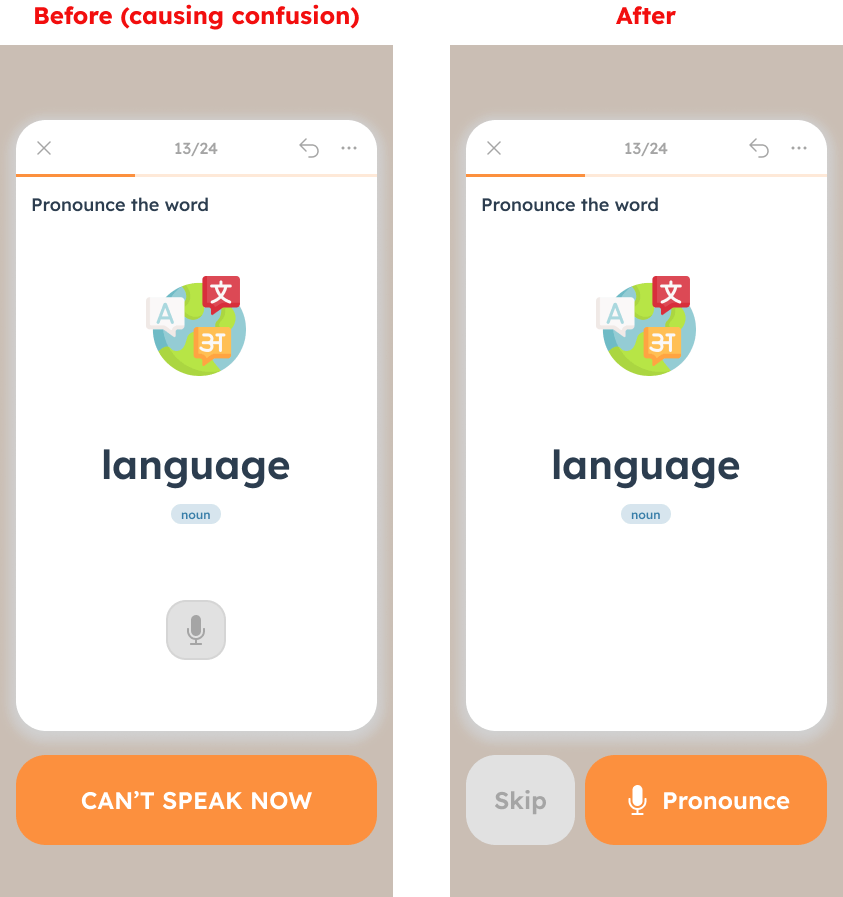
\includegraphics[width=0.60\textwidth]{src/figures/em-testing-pronunciation-before-after.png}
    \caption{Prototype Testing - Pronounce Flashcard Interface Changes}
    \label{fig:em-testing-pronunciation-before-after}
\end{figure}

\begin{table}[ht]
    \centering
    \caption{Results of User Testing Questionnaire}
    \label{tab:questionnaire-results}
    \makebox[\textwidth][c]{
        \begin{tabular}{|p{0.76\textwidth}|c|c|c|c|c|c|c|}
            \hline
            \multicolumn{8}{|l|}{\small A1, A2, A3 = Experienced Users; B1, B2, B3 = Novice Users; Avg = Average} \\
            \multicolumn{8}{|l|}{\small 1 = Strongly Disagree, 2 = Disagree, 3 = Neutral, 4 = Agree, 5 = Strongly Agree} \\
            \hline
            \textbf{Question} & \textbf{A1} & \textbf{A2} & \textbf{A3} & \textbf{B1} & \textbf{B2} & \textbf{B3} & \textbf{Avg} \\
            \hline
            \multicolumn{8}{|l|}{\textbf{Practice Flashcards Experience}} \\
            \hline
            1. The different types of flashcards made practice more engaging & 5 & 5 & 5 & 5 & 5 & 5 & 5.0 \\
            \hline
            2. Each flashcard type's instructions were clear and easy to understand & 5 & 5 & 4 & 4 & 4 & 4 & 4.3 \\
            \hline
            3. The variety in flashcard types helped me learn vocabulary more effectively & 4 & 4 & 5 & 5 & 4 & 4 & 4.3 \\
            \hline
            4. The distribution of different flashcard types felt well-balanced & 4 & 5 & 4 & 5 & 5 & 5 & 4.7 \\
            \hline
            5. The five-stage individual word progress indicator was easy to understand & 5 & 5 & 3 & 4 & 4 & 3 & 4.0 \\
            \hline
            6. Seeing my progress for individual words motivated me to practice more & 4 & 3 & 3 & 4 & 3 & 3 & 3.3 \\
            \hline
            7. The individual word progress indicator's placement was visually clear without being distracting & 2 & 4 & 5 & 5 & 3 & 5 & 4.0 \\
            \hline
            8. I found the progress tracking helpful for understanding my learning journey & 5 & 4 & 5 & 5 & 5 & 4 & 4.7 \\
            \hline
            9. The practice statistics provided useful information about my session & 5 & 4 & 5 & 5 & 4 & 5 & 4.7 \\
            \hline
            10. The celebratory animations made completing practice more rewarding & 5 & 4 & 5 & 5 & 4 & 5 & 4.7 \\
            \hline
            11. The review screen motivated me to complete future practice sessions & 5 & 5 & 5 & 4 & 3 & 5 & 4.5 \\
            \hline
            \multicolumn{8}{|l|}{\textbf{Streak System}} \\
            \hline
            12. The streak system's requirements were clear and easy to understand & 5 & 5 & 4 & 5 & 4 & 5 & 4.7 \\
            \hline
            13. The visual states (active/at risk) effectively communicated streak status & 5 & 5 & 3 & 5 & 4 & 4 & 4.3 \\
            \hline
            14. The celebration screen for maintaining streaks felt rewarding & 5 & 4 & 5 & 5 & 4 & 5 & 4.7 \\
            \hline
            15. The requirement to learn one new word daily feels achievable & 5 & 5 & 5 & 5 & 5 & 5 & 5.0 \\
            \hline
            16. The streak system would help me build a consistent practice habit & 5 & 4 & 5 & 4 & 4 & 5 & 4.5 \\
            \hline
            17. I would be more likely to use the app regularly because of the streak feature & 5 & 5 & 4 & 3 & 4 & 4 & 4.2 \\
            \hline
            \multicolumn{8}{|l|}{\textbf{Overall Experience}} \\
            \hline
            18. The gamification features enhanced my learning experience & 5 & 4 & 5 & 4 & 5 & 5 & 4.7 \\
            \hline
            19. The features felt well-integrated with the app's educational purpose & 4 & 5 & 5 & 5 & 5 & 5 & 4.8 \\
            \hline
            20. The gamification elements maintained my interest without being distracting & 4 & 5 & 5 & 5 & 5 & 5 & 4.8 \\
            \hline
            21. I would recommend this app to others learning English vocabulary & 5 & 5 & 5 & 5 & 5 & 5 & 5.0 \\
            \hline
            22. I would continue using this app for long-term vocabulary learning & 5 & 4 & 5 & 4 & 4 & 5 & 4.5 \\
            \hline
        \end{tabular}
    }
\end{table}